\documentclass[aspectratio=1610]{beamer}

\usepackage{appendixnumberbeamer}
\usepackage[USenglish]{babel}
\usepackage[backend=bibtex,citestyle=authortitle]{biblatex}
\usepackage[scale=2]{ccicons}
\usepackage{graphicx}
\usepackage{listings}
\usepackage{tikz}

% this actually isn't totally hideous:
\usetheme[numbering=counter, progressbar=frametitle, sectionpage=none]{metropolis}
\setbeamertemplate{bibliography item}[text]
\setbeamertemplate{frametitle continuation}{}

\title{Composable Concurrency Models}
\date{November 19, 2016}
\author{Dan Stelljes}

\bibliography{references}

\AtEveryBibitem{\clearfield{note}}
\AtEveryBibitem{\clearfield{url}}

\begin{document}
  \maketitle

  \section{Introduction}

  \begin{frame}
    \centering
    \resizebox{0.8\linewidth}{!}{\begin{tikzpicture}
  \onslide<1->{
    \node at (0,0) {
      
\includegraphics[width=300pt]{browser}
    };
  }

  \onslide<2>{
    \path (-2.25,2.75) [draw=none, fill=darkgray, opacity=0.75] ellipse (60pt and 25pt);
    \node [text=white] at (-2.25,2.75) {
      Multiple tabs
    };

    \draw (2.25,2.25) [draw=none, fill=darkgray, opacity=0.75] ellipse (60pt and 25pt);
    \node [text=white] at (2.25,2.25) {
      Suggestions
    };

    \draw (0,0.5) [draw=none, fill=darkgray, opacity=0.75] ellipse (60pt and 25pt);
    \node [text=white] at (0,0.5) {
      Page rendering
    };

    \draw (-3,-1.5) [draw=none, fill=darkgray, opacity=0.75] ellipse (60pt and 25pt);
    \node [text=white] at (-3,-1.5) {
      Event handling
    };

    \draw (2.5,-1.5) [draw=none, fill=darkgray, opacity=0.75] ellipse (60pt and 25pt);
    \node [text=white] at (2.5,-1.5) {
      Background processes
    };
  }

  \onslide<3>{
    \node at (0,-0.62) {
      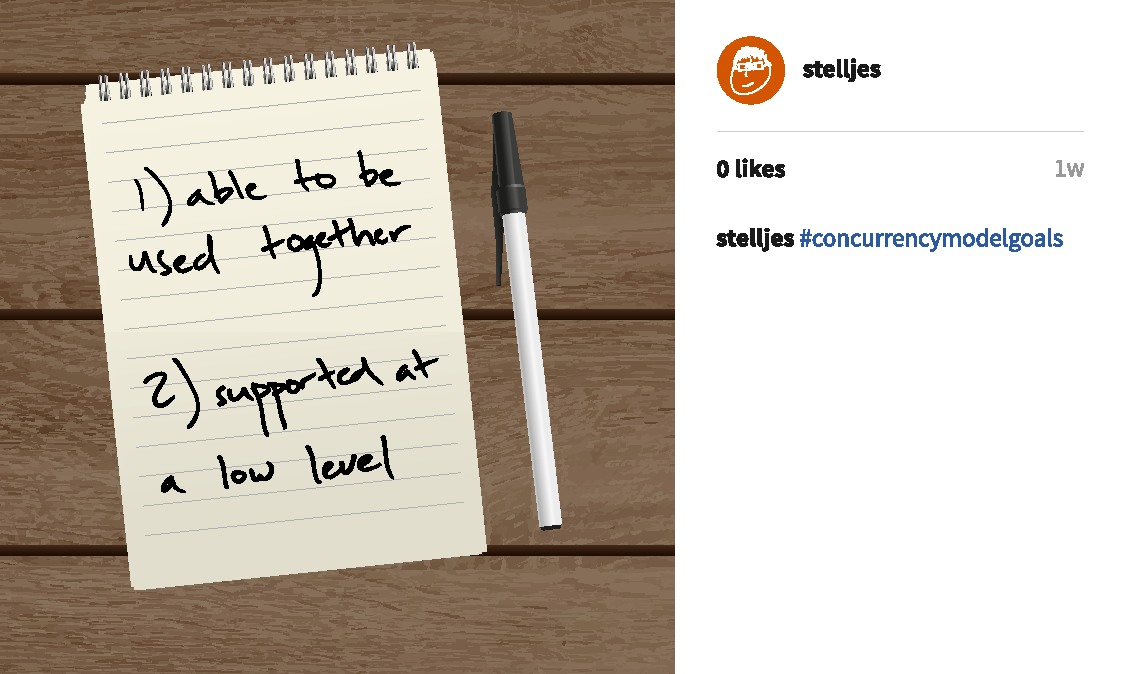
\includegraphics[width=220pt]{goals}
    };
  }
\end{tikzpicture}
}
  \end{frame}

  \section{Background}

  \subsection{Concurrency}

  \begin{frame}
    \frametitle{Concurrency}

    \textbf{The ``happens before'' ($\rightarrow$) relation~\footcite{Lamport1977}}

    $A \rightarrow B$ if one of the following is true:

    \begin{enumerate}
      \item $A$ and $B$ are operations in the same thread and $A$ occurs before $B$.
      \item $A$ is the sending of a message by one thread and $B$ is the receipt of the same message by another thread.
    \end{enumerate}

    If $A \rightarrow B$ and $B \rightarrow C$, then $A \rightarrow C$.

    $A$ and $B$ are said to be concurrent if $A \nrightarrow B$ and $B \nrightarrow A$.
  \end{frame}

  \subsection{Complications}

  \begin{frame}
    \frametitle{Complications}

    \begin{itemize}
      \onslide<1->{
        \item \textbf{Sequential program:} Does the order of operations yield a correct result?
      }

      \vfill

      \onslide<2->{
        \item \textbf{Concurrent program:} Does \emph{every possible} order of operations yield a correct result?
      }
    \end{itemize}
  \end{frame}

  \begin{frame}
    \frametitle{Complications}
    \centering

    \textbf{Single thread:}
    \vfill
    \resizebox{0.9\linewidth}{!}{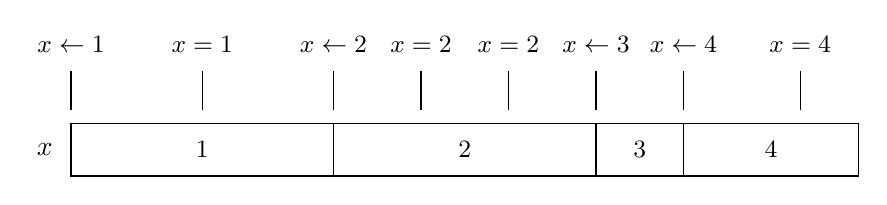
\begin{tikzpicture}
  \node at (-5.333,0) { $x$ };

  \draw (-5,-0.333) rectangle (-1.667,0.333) node [midway] { \small $1$ };
  \draw (-1.667,-0.333) rectangle (1.667,0.333) node [midway] { \small $2$ };
  \draw (1.667,-0.333) rectangle (2.778,0.333) node [midway] { \small $3$ };
  \draw (2.778,-0.333) rectangle (5,0.333) node [midway] { \small $4$ };

  \draw (-5,0.5) -- (-5,1) node [above=3pt] { \small $x \leftarrow 1$ };
  \draw (-3.333,0.5) -- (-3.333,1) node [above=3pt] { \small $x = 1$ };

  \draw (-1.667,0.5) -- (-1.667,1) node [above=3pt] { \small $x \leftarrow 2$ };
  \draw (-0.555,0.5) -- (-0.555,1) node [above=3pt] { \small $x = 2$ };
  \draw (0.555,0.5) -- (0.555,1) node [above=3pt] { \small $x = 2$ };

  \draw (1.667,0.5) -- (1.667,1) node [above=3pt] { \small $x \leftarrow 3$ };

  \draw (2.778,0.5) -- (2.778,1) node [above=3pt] { \small $x \leftarrow 4$ };
  \draw (4.26,0.5) -- (4.26,1) node [above=3pt] { \small $x = 4$ };
\end{tikzpicture}
}
  \end{frame}

  \begin{frame}
    \frametitle{Complications}
    \centering

    \textbf{Multiple threads:}
    \vfill
    \resizebox{0.9\linewidth}{!}{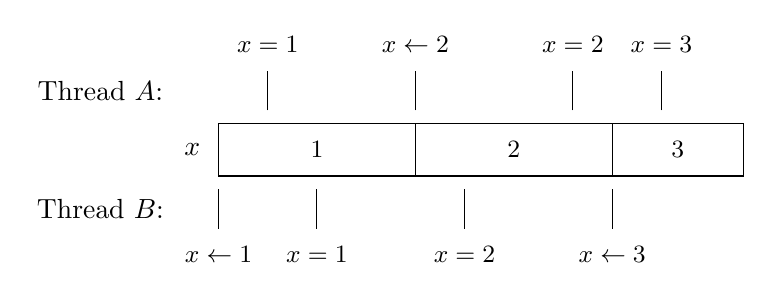
\begin{tikzpicture}
  \node at (-6.5,0.75) { Thread $A$: };
  \node at (-6.5,-0.75) { Thread $B$: };
  \node at (-5.333,0) { $x$ };

  \draw (-5,-0.333) rectangle (-2.5,0.333) node [midway] { \small $1$ };
  \draw (-2.5,-0.333) rectangle (0,0.333) node [midway] { \small $2$ };
  \draw (0,-0.333) rectangle (1.667,0.333) node [midway] { \small $3$ };

  \draw (-5,-0.5) -- (-5,-1) node [below=3pt] { \small $x \leftarrow 1$ };
  \draw (-4.375,0.5) -- (-4.375,1) node [above=3pt] { \small $x = 1$ };
  \draw (-3.75,-0.5) -- (-3.75,-1) node [below=3pt] { \small $x = 1$ };

  \draw (-2.5,0.5) -- (-2.5,1) node [above=3pt] { \small $x \leftarrow 2$ };
  \draw (-1.875,-0.5) -- (-1.875,-1) node [below=3pt] { \small $x = 2$ };
  \draw (-0.5,0.5) -- (-0.5,1) node [above=3pt] { \small $x = 2$ };

  \draw (0,-0.5) -- (0,-1) node [below=3pt] { \small $x \leftarrow 3$ };
  \draw (0.625,0.5) -- (0.625,1) node [above=3pt] { \small $x = 3$ };
\end{tikzpicture}
}
  \end{frame}

  \begin{frame}
    \frametitle{Complications}

    \centering
    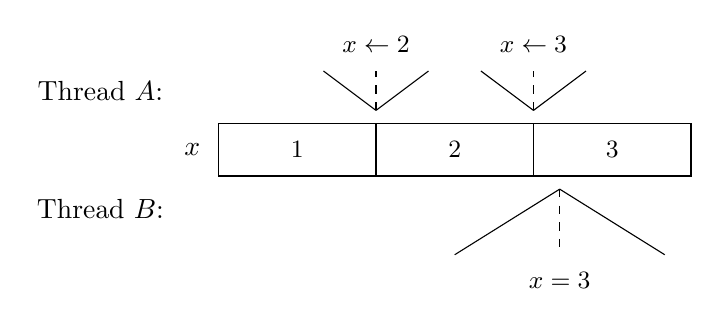
\begin{tikzpicture}
  \node at (-4.5,0.75) { Thread $A$: };
  \node at (-4.5,-0.75) { Thread $B$: };
  \node at (-3.333,0) { $x$ };

  \draw (-3,-0.333) rectangle (-1,0.333) node [midway] { \small $1$ };
  \draw (-1,-0.333) rectangle (1,0.333) node [midway] { \small $2$ };
  \draw (1,-0.333) rectangle (3,0.333) node [midway] { \small $3$ };

  \draw (-1.667,1) -- (-1,0.5) (-1,0.5) -- (-0.333,1);
  \draw [dashed] (-1,0.5) -- (-1,1) node [above=3pt] { \small $x \leftarrow 2$ };

  \draw (0.333,1) -- (1,0.5) (1,0.5) -- (1.667,1);
  \draw [dashed] (1,0.5) -- (1,1) node [above=3pt] { \small $x \leftarrow 3$ };

  \draw (0,-1.333) -- (1.333,-0.5) (1.333,-0.5) -- (2.667,-1.333);
  \draw [dashed] (1.333,-0.5) -- (1.333,-1.333) node [below=3pt] { \small $x = 3$ };
\end{tikzpicture}

  \end{frame}

  \subsection{Consistency models}

  \begin{frame}
    \frametitle{Linearizability}

    \begin{figure}
      \centering
      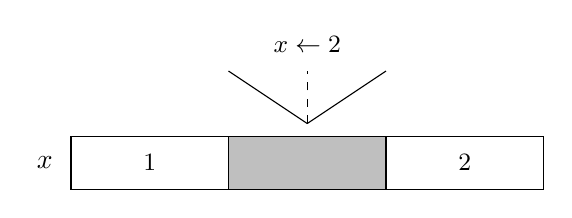
\begin{tikzpicture}
  \node at (-3.333,0) { $x$ };

  \draw (-3,-0.333) rectangle (-1,0.333) node [midway] { \small $1$ };
  \draw [fill=lightgray] (-1,-0.333) rectangle (1,0.333);
  \draw (1,-0.333) rectangle (3,0.333) node [midway] { \small $2$ };

  \draw (-1,1.167) -- (0,0.5) (0,0.5) -- (1,1.167);
  \draw [dashed] (0,0.5) -- (0,1.167) node [above=3pt] { \small $x \leftarrow 2$ };
\end{tikzpicture}

    \end{figure}

    \vfill

    \begin{itemize}
      \item Linearizability guarantees that the completion of an operation on a single object will appear to be instantaneous.
      \item The results of a linearizable operation will be visible as soon as the operation is complete.
    \end{itemize}
  \end{frame}

  \begin{frame}
    \frametitle{Serializability}

    \begin{figure}
      \centering
      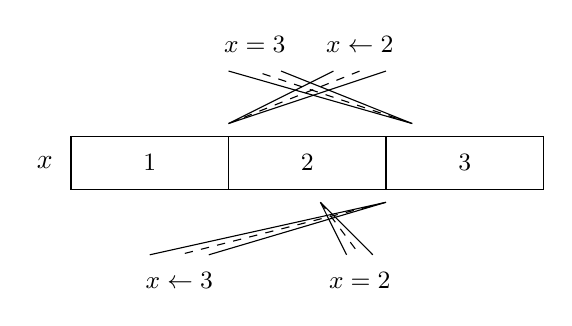
\begin{tikzpicture}
  \node at (-3.333,0) { $x$ };

  \draw (-3,-0.333) rectangle (-1,0.333) node [midway] { \small $1$ };
  \draw (-1,-0.333) rectangle (1,0.333) node [midway] { \small $2$ };
  \draw (1,-0.333) rectangle (3,0.333) node [midway] { \small $3$ };

  \draw (0.333,1.167) -- (-1,0.5) (-1,0.5) -- (1,1.167);
  \draw [dashed] (-1,0.5) -- (0.667,1.167) node [above=3pt] { \small $x \leftarrow 2$ };

  \draw (0.5,-1.167) -- (0.167,-0.5) (0.167,-0.5) -- (0.833,-1.167);
  \draw [dashed] (0.167,-0.5) -- (0.667,-1.167) node [below=3pt] { \small $x = 2$ };

  \draw (-2,-1.167) -- (1,-0.5) (1,-0.5) -- (-1.25,-1.167);
  \draw [dashed] (1,-0.5) -- (-1.625, -1.167) node [below=3pt] { \small $x \leftarrow 3$ };

  \draw (-1,1.167) -- (1.333,0.5) (1.333,0.5) -- (-0.333,1.167);
  \draw [dashed] (1.333,0.5) -- (-0.667,1.167) node [above=3pt] { \small $x = 3$ };
\end{tikzpicture}

    \end{figure}

    \vfill

    \begin{itemize}
      \item Serializability guarantees that operations can occur in any order as long as an equivalent sequential ordering exists.
      \item While a serializable set of operations is being executed, it appears to be the only set of operations being executed.
    \end{itemize}
  \end{frame}

  \begin{frame}
    \frametitle{Strict serializability}

    \begin{itemize}
      \item Linearizability \emph{and} serializability yield strict serializability, which guarantees both consistency and isolation.
    \end{itemize}

    \vfill

    \textbf{Strict serializability~\footcite{Herlihy1990}}

    An ordering of operations is equivalent to some sequential ordering and that ordering corresponds to the order of execution in real time.
  \end{frame}

  \section{Concurrency models}

  \subsection{Atomic variables}

  \begin{frame}
    \frametitle{Atomic variables}

    \begin{columns}
      \begin{column}{0.5\textwidth}
        \centering
        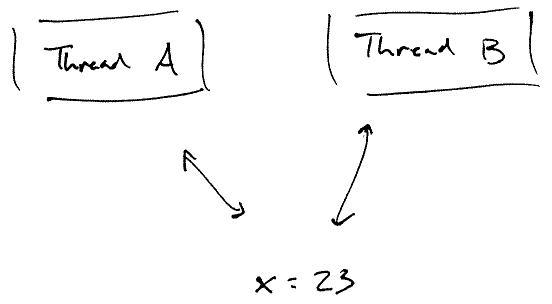
\includegraphics[width=160pt]{../figures/nonatomic}
      \end{column}
      \hfill
      \begin{column}{0.5\textwidth}
        $x = 23$

        \begin{enumerate}
          \item $A$ reads $x$
          \item $B$ reads $x$
          \item $A$ increments value
          \item $A$ writes incremented value to $x$
          \item $B$ increments value
          \item $B$ writes incremented value to $x$
        \end{enumerate}

        $x = 24$
      \end{column}
    \end{columns}
  \end{frame}

  \begin{frame}
    \frametitle{Atomic variables}

    \begin{columns}
      \begin{column}{0.5\textwidth}
        \centering
        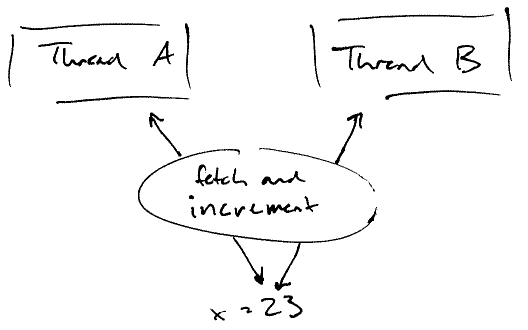
\includegraphics[width=160pt]{../figures/atomic}
      \end{column}
      \hfill
      \begin{column}{0.5\textwidth}
        $x = 23$

        \begin{enumerate}
          \item $A$ calls \textsc{fetch-and-increment} on $x$
          \item $B$ calls \textsc{fetch-and-increment} on $x$
        \end{enumerate}

        $x = 25$
      \end{column}
    \end{columns}
  \end{frame}

  \begin{frame}
    \frametitle{Atomic variables}
    \centering

    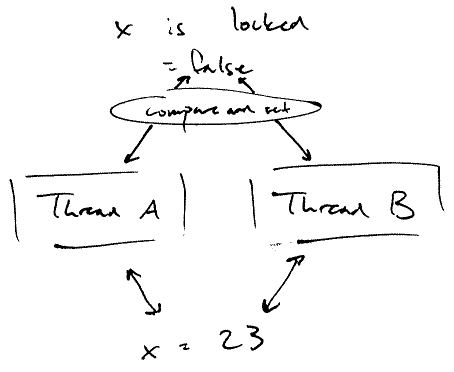
\includegraphics[width=220pt]{../figures/lock}
  \end{frame}

  \begin{frame}
    \frametitle{Atomic variables}
    \centering

    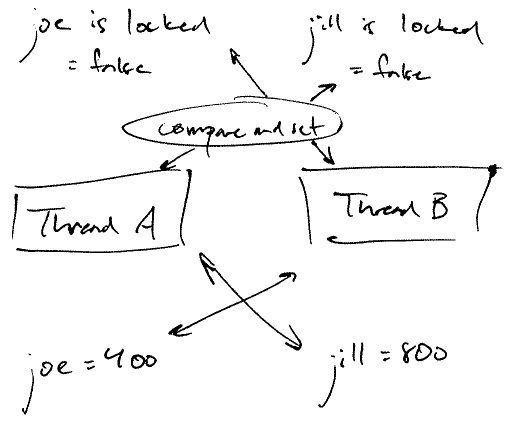
\includegraphics[width=220pt]{../figures/multiple-locks}
  \end{frame}

  \subsection{Transactional memory}

  \begin{frame}
    \frametitle{Transactional memory}
    \centering

    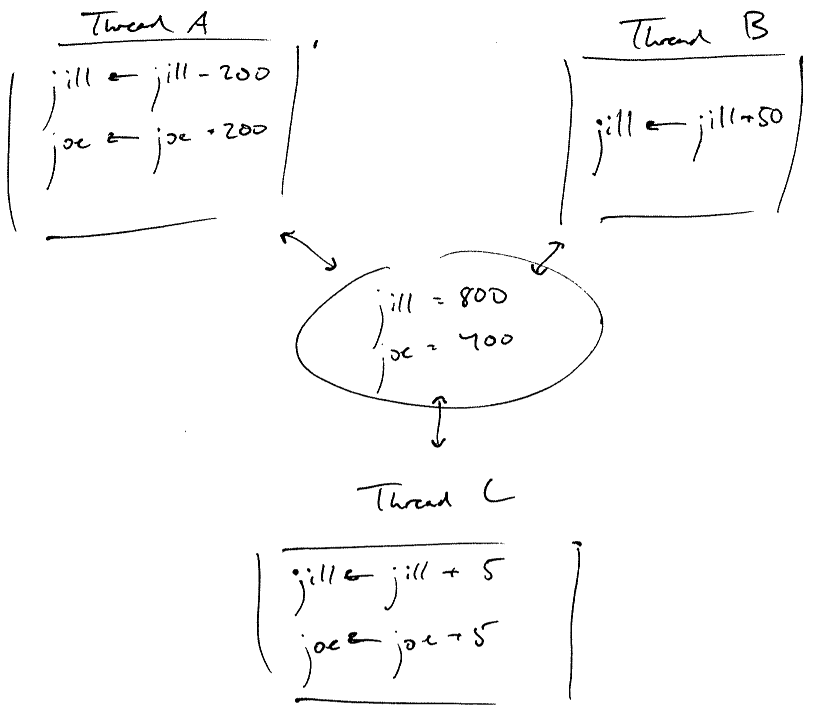
\includegraphics[width=220pt]{../figures/stm}
  \end{frame}

  \begin{frame}
    \frametitle{Transactional memory}

    Software transactional memory (STM) is an optimistic approach to working with shared memory:~\footcite{Shavit1995}

    \begin{enumerate}
      \item A thread writes to a shared memory location, keeping track of the transaction in a log.
      \item If there are conflicting changes at the end of the transaction, the transaction is aborted and retried.
      \item If there are no conflicts, the changes are committed and become visible.
    \end{enumerate}
  \end{frame}

  \subsection{Communicating threads}

  \begin{frame}
    \frametitle{Communicating threads}
    \centering

    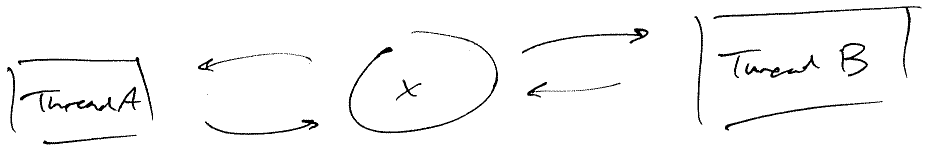
\includegraphics[width=220pt]{../figures/agent}
    \vfill
    \textbf{Agents:} An isolated thread handles all operations on an object.~\footcite{Swalens2014}
  \end{frame}

  \begin{frame}
    \frametitle{Communicating threads}
    \centering

    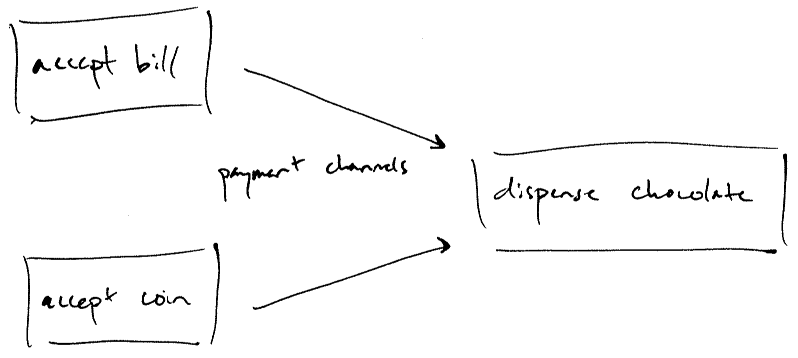
\includegraphics[width=220pt]{../figures/csp}
    \vfill
    \textbf{Communicating sequential processes (CSP):} Independent threads communicate synchronously through predefined channels.~\footcite{Hoare1978}
  \end{frame}

  \begin{frame}
    \frametitle{Communicating threads}
    \centering

    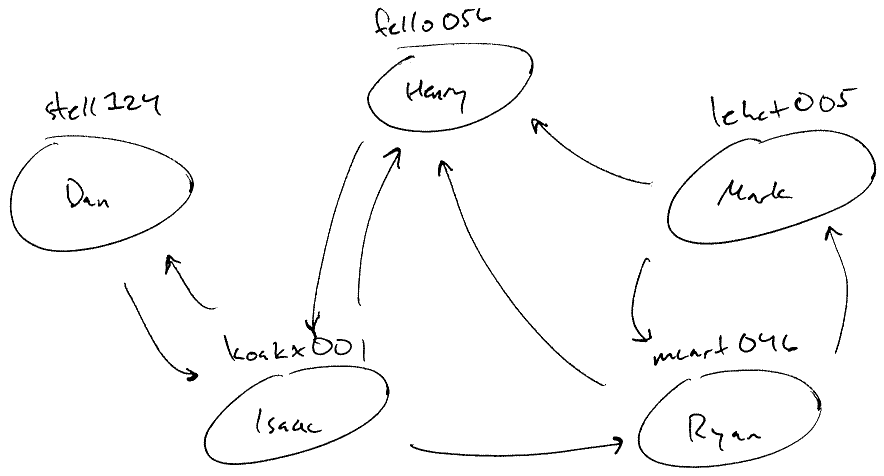
\includegraphics[width=220pt]{../figures/actor}
    \vfill
    \textbf{The actor model:} Independent threads send messages to known addresses.~\footcite{Agha1986}
  \end{frame}

  \section{Composability challenges}

  \begin{frame}
    \frametitle{Composability criteria}

    \textbf{How do we know that models are composable?~\footcite{Swalens2014}}

    \begin{itemize}
      \item Safety: ``Nothing bad will happen!'' (The output of a program or algorithm will not be incorrect.)
      \item Liveness: ``Something will eventually happen!'' (The program or algorithm will terminate.)
    \end{itemize}

    Two models are composable if using them within each other doesn't compromise safety or liveness.
  \end{frame}

  \begin{frame}
    \frametitle{Composability criteria}
    \centering

    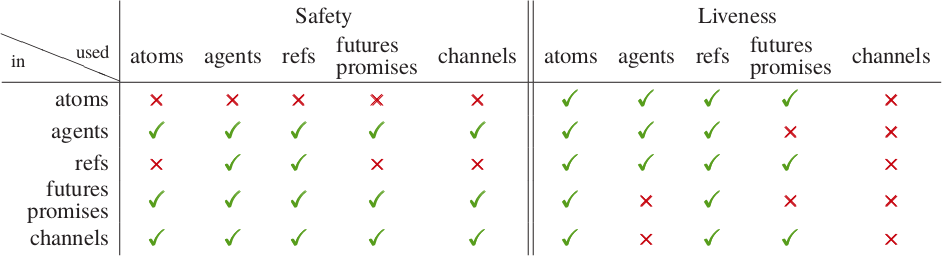
\includegraphics[width=360pt]{../figures/clojure-survey}
  \end{frame}

  \begin{frame}
    \frametitle{Possible conflicts}

    \begin{itemize}
      \onslide<1->{
        \item A model reexecutes code containing another model that performs an irrevocable action.
      }
      \vfill
      \onslide<2->{
        \item A model reexecutes code that causes the reexecution to continually happen.
      }
      \vfill
      \onslide<3->{
        \item A model that supports blocking operations is used within a model that does not support blocking operations.
      }
      \vfill
      \onslide<4->{
        \item A model does not guarantee safety or liveness by design, making composability impossible.
      }
    \end{itemize}
  \end{frame}

  \begin{frame}
    \frametitle{Conclusions}

    \begin{itemize}
      \onslide<1->{
        \item The language may ensure that some bad interactions don't happen.
      }
      \vfill
      \onslide<2->{
        \item Sometimes, it's best to just use a different concurrency model.
      }
      \vfill
      \onslide<3->{
        \item Future work would identify common ``building blocks'' (thread creation, message passing, etc.) that could be composed to express existing concurrency models and combinations of models.
      }
    \end{itemize}
  \end{frame}

  \section{Unifying abstractions}

  \subsection{Ownership-based meta-object protocol}

  \begin{frame}
    \frametitle{Proposed abstractions}

    \textbf{What characteristics should a unifying abstraction have?}~\footcite{Marr2012}

    \begin{itemize}
      \onslide<1->{
        \item Ownership: All objects are owned by something, so ownership should be supported in a way that supports regulated access.
      }
      \vfill
      \onslide<2->{
        \item Managed mutation and execution: The owner of an object should determine how the object should be read and modified.
      }
      \vfill
      \onslide<3->{
        \item Leveled access: Threads should either have model-level access or abstraction-level access.
      }
      \vfill
      \onslide<4->{
        \item Enforceability: The abstraction should be able to enforce all model rules.
      }
    \end{itemize}
  \end{frame}

  \begin{frame}
    \frametitle{Ownership-based meta-object protocol}

    \centering

    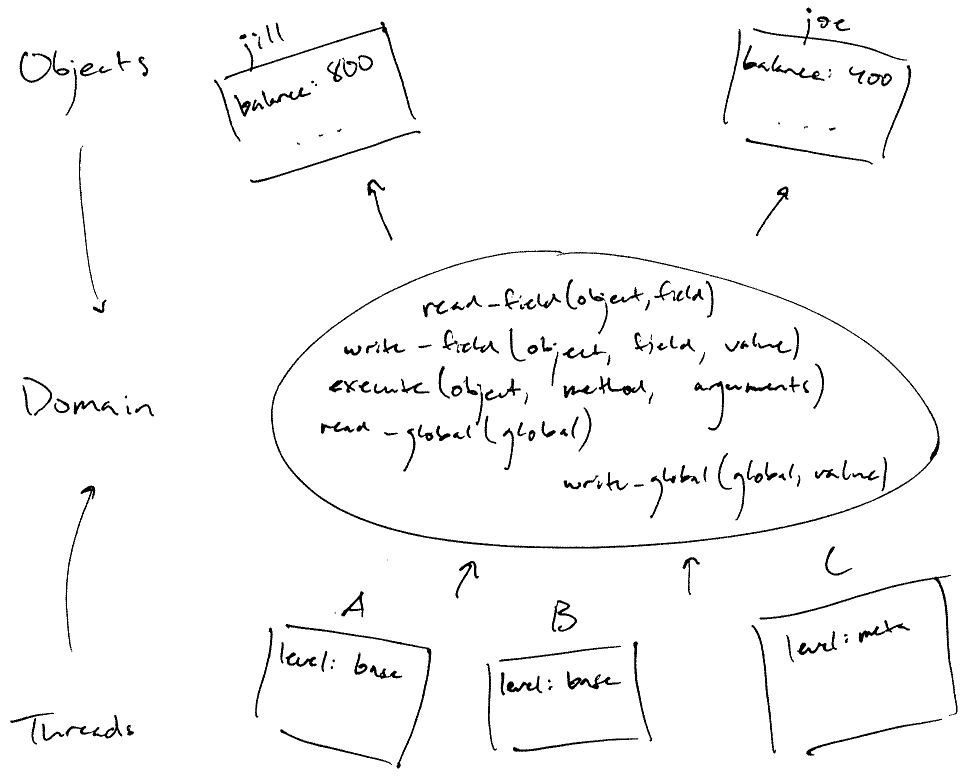
\includegraphics[width=250pt]{../figures/obmop-simple.png}
  \end{frame}

  \begin{frame}
    \frametitle{Conclusions}

    \begin{itemize}
      \onslide<1->{
        \item An abstraction like the OBMOP must be implemented at a low level to achieve acceptable performance.
      }
      \vfill
      \onslide<2->{
        \item The OBMOP has some limitations: The owner is the only entity that enforces rules, and the abstraction doesn't guarantee things like freedom from deadlock.
      }
      \vfill
      \onslide<3->{
        \item This approach has potential: The authors were able to implement STM, CSP, agents, and actors in less than 500 total lines of code.
      }
    \end{itemize}
  \end{frame}

  \begin{frame}[standout]
    \centering
    Thanks to Elena Machkasova, K.K. Lamberty, and Matthew Justin for their guidance and suggestions.
    \vfill
    \href{https://github.com/dstelljes/senior-sem}{github.com/dstelljes/senior-sem}
    \vfill
    \ccbyncsa{}
  \end{frame}

  \appendix{}

  \begin{frame}[allowframebreaks]
    \frametitle{References}

    \printbibliography{}
  \end{frame}

\end{document}
